%\documentclass[10pt, a4paper]{article}

%\input{../template/preamble.tex}

%\usepackage{moreverb}

%\usepackage{a4}
%\usepackage{times}

%\date{}

%\begin{document}

%\title{Performance Evaluation of Language Analysers}

%%%%%%%%%%%%%%%%%%%%%%%%%%%%%%%%%%%%%%%%%%%%%%%%%%%%%%%%%%%%%%%%%%%%%%%%%%%%%
%
% gui.tex
%
% hamish, 25/8/1
%
% $Id: gui.tex,v 1.32 2005/04/25 16:28:17 diana Exp $
%
%%%%%%%%%%%%%%%%%%%%%%%%%%%%%%%%%%%%%%%%%%%%%%%%%%%%%%%%%%%%%%%%%%%%%%%%%%%%%


%%%%%%%%%%%%%%%%%%%%%%%%%%%%%%%%%%%%%%%%%%%%%%%%%%%%%%%%%%%%%%%%%%%%%%%%%%%%%
\chapt[chap:eval]{Performance Evaluation of Language Analysers}
\markboth{Performance Evaluation of Language Analysers}{Performance Evaluation of Language Analysers}
%%%%%%%%%%%%%%%%%%%%%%%%%%%%%%%%%%%%%%%%%%%%%%%%%%%%%%%%%%%%%%%%%%%%%%%%%%%%%

%%%% qqqqqqqqqqqqqqqqqqqqqqqqq %%%%
\ifprintedbook
\else
\begin{quote}
When you can measure what you are speaking about, and
express it in numbers, you know something about it; but when
you cannot measure it, when you cannot express it in numbers, your
knowledge is of a meager and unsatisfactory kind: it
may be the beginning of knowledge, but you have scarcely in your
thoughts advanced to the stage of science. (Kelvin)

Not everything that counts can be counted, and not everything that can
be counted counts. (Einstein) 
\end{quote}
\fi
%%%% qqqqqqqqqqqqqqqqqqqqqqqqq %%%%

%GATE provides two useful tools for automatic evaluation: the Annotation Diff
%tool and the Corpus benchmark Tool. 

GATE provides a variety of tools for automatic evaluation. The Annotation Diff
tool compares two annotation sets within a document. Corpus QA extends Annotation
Diff to an entire corpus. The Corpus Benchmark tool also provides
functionality for comparing annotation sets over an entire corpus. Additionally,
two plugins cover similar functionality; one implements inter-annotator
agreement, and the other, the balanced distance metric.

These tools are particularly useful not just as a final measure of performance,
but as a tool to aid system development by tracking progress and evaluating the
impact of changes as they are made. Applications include evaluating the success
of a machine learning or language engineering application by comparing its
results to a gold standard and also comparing annotations prepared by two
human annotators to each other to ensure that the annotations are reliable.

This chapter begins by introducing the concepts and metrics relevant, before
describing each of the tools in turn.

% The
%Annotation Diff tool enables automated performance measurement and
%visualisation of the results, while the corpus benchmark tool enables the
%tracking of a system's progress and regression testing.

%%%%%%%%%%%%%%%%%%%%%%%%%%%%%%%%%%%%%%%%%%%%%%%%%%%%%%%%%%%%%%%%%%%%%%%%%%%%%
\sect[sec:eval:metrics]{Metrics for Evaluation in Information Extraction}
%%%%%%%%%%%%%%%%%%%%%%%%%%%%%%%%%%%%%%%%%%%%%%%%%%%%%%%%%%%%%%%%%%%%%%%%%%%%%

When we evaluate the performance of a processing resource such as tokeniser, POS
tagger, or a whole application, we usually have a human-authored `gold standard'
against which to compare our software. However, it is not always easy or obvious
what this gold standard should be, as different people may have different
opinions about what is correct. Typically, we solve this problem by using more
than one human annotator, and comparing their annotations. We do this by
calculating inter-annotator agreement (IAA), also known as inter-rater reliability.

IAA can be used to assess how difficult a task is. This is based on the argument
that if two humans cannot come to agreement on some annotation, it is unlikely
that a computer could ever do the same annotation `correctly'. Thus, IAA can be
used to find the ceiling for computer performance.

There are many possible metrics for reporting IAA, such as Cohen's Kappa,
prevalence, and bias \cite{Eugenio04}. Kappa is the best metric for IAA when all
the annotators have identical exhaustive sets of questions on which they might
agree or disagree. In other words, it is a classification task. This could be a
task like `are these names male or female names'. However, sometimes there is
disagreement about the set of questions, e.g. when the annotators themselves
determine which text spans they ought to annotate, such as in named entity
extraction. That could be a task like `read over this text and mark up all
references to politics'. When annotators determine their own sets of questions,
it is appropriate to use precision, recall, and F-measure to report IAA.
Precision, recall and F-measure are also appropriate choices when assessing
performance of an automated application against a trusted gold standard.

In this section, we will first introduce some relevant terms, before outlining
Cohen's Kappa and similar measures, in Section~\ref{sec:eval:kappa}. We will then
introduce precision, recall and F-measure in Section~\ref{sec:eval:prf}.

%%%%%%%%%%%%%%%%%%%%%%%%%%%%%%%%%%%%%%%%%%%%%%%%%%%%%%%%%%%%%%%%%%%%%%
\subsect[sec:eval:benchmarktoolrelation]{Annotation Relations}
%%%%%%%%%%%%%%%%%%%%%%%%%%%%%%%%%%%%%%%%%%%%%%%%%%%%%%%%%%%%%%%%%%%%%%

Before introducing the metrics we will use in this \chapthing, we will first
outline the ways in which annotations can relate to each other. These ways of
comparing annotations to each other are used to determine the counts that then go
into calculating the metrics of interest. Consider a document with two annotation
sets upon it. These annotation sets might for example be prepared by two human
annotators, or alternatively, one set might be produced by an automated system
and the other might be a trusted gold standard. We wish to assess the extent to
which they agree. We begin by counting incidences of the following relations:

\begin{description}

\item[Coextensive] Two annotations are coextensive if they hit the same span of
text in a document. Basically, both their start and end offsets are equal.

\item[Overlaps] Two annotations overlap if they share a common span of text.

\item[Compatible] Two annotations are compatible if they are coextensive and if
the features of one (usually the ones from the key) are included in
the features of the other (usually the response).

\item[Partially Compatible] Two annotations are partially compatible if they
overlap and if the features of one (usually the ones from the key) are included in
the features of the other (response).

\item[Missing] This applies only to the key annotations. A key annotation is
missing if either it is not coextensive or overlapping, orif one or more
features are not included in the response annotation.

\item[Spurious] This applies only to the response annotations. A response
annotation is spurious if either it is not coextensive or overlapping, or if one or
more features from the key are not included in the response
annotation.

\end{description}

%%%%%%%%%%%%%%%%%%%%%%%%%%%%%%%%%%%%%%%%%%%%%%%%%%%%%%%%%%%%%%%%%%%%%%%%%%%%%
\subsect[sec:eval:kappa]{Cohen's Kappa}
%%%%%%%%%%%%%%%%%%%%%%%%%%%%%%%%%%%%%%%%%%%%%%%%%%%%%%%%%%%%%%%%%%%%%%%%%%%%%

The three commonly used IAA measures are {\em observed agreement}, {\em specific agreement}, 
and {\em Kappa ($\kappa$)} \cite{Hripcsak02}. Those measures can be 
calculated from a contingency table, which lists the numbers of instances of 
agreement and disagreement between two annotators on each category. To explain the 
IAA measures, a general contingency table for two categories {\em cat1} and {\em cat2}
 is shown in Table \ref{table:iaa-kappa:contingency}.

\begin{table}[hbt]
{\centering
\begin{tabular}{|l|cc|c|} 
\hline
   & Annotator-2 & & \\
\hline
Annotator-1  & cat1 & cat2 & marginal sum\\
\hline
 cat1& a & b & a+b\\ 
cat2 & c & d & c+d\\
\hline
marginal sum & a+c & b+d &a+b+c+d\\
 \hline
\end{tabular}\par}
\caption{Contingency table for two-category problem}
\label{table:iaa-kappa:contingency}
\end{table}


{\bf Observed agreement} is the portion of the instances on which the 
annotators agree. For the two annotators and two categories as shown in
 Table \ref{table:iaa-kappa:contingency}, it is defined as
\begin{equation}
A_{o} = \frac{a+d}{a+b+c+d}
\end{equation}
The extension of the above formula to more than two categories is 
straightforward. The extension to more than two annotators is usually taken 
as the mean of the pair-wise agreements \cite{Fleiss75}, which is the average agreement 
across all possible pairs of annotators. 
An alternative compares each annotator with the majority opinion of the others 
\cite{Fleiss75}.

However, the observed agreement has two shortcomings. One is that a certain 
amount of agreement is expected by chance. The Kappa measure is a chance-corrected 
agreement. Another is that it sums up the agreement on all the categories, but 
the agreements on each category may differ. Hence the category specific agreement 
is needed.

{\bf Specific agreement} quantifies the degree of agreement for each of the categories 
separately. For example, the specific agreement for the two categories list in 
Table \ref{table:iaa-kappa:contingency} is the following, respectively,
\begin{equation}
A_{cat1} = \frac{2a}{2a+b+c}; \ \ \
A_{cat2} = \frac{2d}{b+c+2d}
\end{equation}

{\bf Kappa} is defined as the observed agreements $A_{o}$ minus the agreement 
expected by chance $A_{e}$ and is normalized as a number between -1 and 1.
\begin{equation}
\kappa =\frac{A_{o}-A_{e}}{1-A_{e}}
\end{equation}

$\kappa=1$ means perfect agreements, $\kappa=0$ means the agreement is equal to 
chance, $\kappa=-1$ means `perfect' disagreement.

There are two different ways of computing the chance agreement $A_{e}$ (for a
detailed explanations about it see \cite{Eugenio04}; however, a quick outline
will be given below). The Cohen's Kappa is based on the individual distribution
of each annotator, while the Siegel \& Castellan's Kappa is based on the
assumption that all the annotators have the same distribution. The former is more
informative than the latter and has been used widely.

Let us consider an example:

\begin{table}[hbt]
{\centering
\begin{tabular}{|l|cc|c|} 
\hline
   & Annotator-2 & & \\
\hline
Annotator-1  & cat1 & cat2 & marginal sum\\
\hline
 cat1& 1 & 2 & 3\\ 
cat2 & 3 & 4 & 7\\
\hline
marginal sum & 4 & 6 &10\\
 \hline
\end{tabular}\par}
\caption{Example contingency table for two-category problem}
\label{table:iaa-kappa:contingencyex}
\end{table}

{\bf Cohen's Kappa} requires that the expected agreement be calculated as
follows. Divide marginal sums by the total to get the portion of the instances
that each annotator allocates to each category. Multiply annotator's
proportions together to get the likelihood of chance agreement, then total
these figures. Table~\ref{table:iaa-kappa:cohens} gives a worked example.

\begin{table}[hbt]
{\centering
\begin{tabular}{|l|l|l|l|} 
\hline
   & Annotator-1 & Annotator 2 & Multiplied \\
\hline
cat1 & 3 / 10 = 0.3 & 4 / 10 = 0.4 & 0.12 \\ 
cat2 & 7 / 10 = 0.7 & 6 / 10 = 0.6 & 0.42 \\
\hline
Total & & & 0.54 \\
\hline
\end{tabular}\par}
\caption{Calculating Expected Agreement for Cohen's Kappa}
\label{table:iaa-kappa:cohens}
\end{table}

The formula can easily be extended to more than two categories.

{\bf Siegel \& Castellan's Kappa} is applicable for any number of annotators.
Siegel \& Castellan's Kappa for two annotators is also known as Scott's Pi (see
\cite{Lombard02}). It differs from Cohen's Kappa only in how the expected
agreement is calculated. Table~\ref{table:iaa-kappa:scotts} shows a worked
example. Annotator totals are added together and divided by the number of
decisions to form joint proportions. These are then squared and totalled.

\begin{table}[hbt]
{\centering
\begin{tabular}{|l|l|l|l|l|l|} 
\hline
   & Ann-1 & Ann-2 & Sum & Joint Prop &
   JP-Squared \\
\hline
cat1 & 3 & 4 & 7 & 7/20 & 49/400=0.1225 \\ 
cat2 & 7 & 6 & 13 & 13/20 & 169/400=0.4225 \\ 
\hline
Total & & & & & 218/400 = 0.545 \\
\hline
\end{tabular}\par}
\caption{Calculating Expected Agreement for Siegel \& Castellan's Kappa
(Scott's Pi)}
\label{table:iaa-kappa:scotts}
\end{table}

The Kappa suffers from the prevalence problem which arises because imbalanced
distribution of categories in the data increases $A_{e}$. The prevalence problem
can be alleviated by reporting the positive and negative specified  agreement on
each category besides the Kappa \cite{ Hripcsak02, Eugenio04}. In addition, the
so-called bias problem affects the Cohen's Kappa, but not S\&C's. The bias
problem arises as one annotator prefers one particular category more than another
annotator. \cite{Eugenio04} advised to compute the S\&C's Kappa and the specific
agreements along with the Cohen's Kappa in order to handle these problems.

Despite the problem mentioned above, the Cohen's Kappa remains a popular IAA measure. 
Kappa can be used for more than two annotators based on pair-wise figures, e.g. the mean
of all the pair-wise Kappa as an overall Kappa measure. The Cohen's Kappa can also be
extended to the case of more than two annotators by using the following single 
formula  \cite{Davies82}
\begin{equation}
\kappa = 1-\frac{IJ^{2}-\sum_{i}\sum_{c}Y_{ic}^{2}}
{I(J(J-1)\sum_{c}(p_{c}(1-p_{c}))+ \sum_{c}\sum_{j}(p_{cj}-p_{c})^2)}
\end{equation}
Where $I$ and $J$ are the number of instances and annotators, respectively; $Y_{ic}$ 
is the number of annotators who assigns the category $c$ to the instance $I$; $p_{cj}$ 
is the probability of the annotator $j$ assigning category $c$; $p_{c}$ is the 
probability of assigning category by all annotators (i.e. averaging $p_{cj}$  
over all annotators).

The Krippendorff's alpha, another variant of Kappa, differs only slightly from
the S\&C's Kappa on nominal category problem (see \cite{Carletta96, Eugenio04}).

However, note that the Kappa (and the observed agreement) is not applicable to some
tasks. Named entity annotation is  one such task
\cite{Hripcsak05}. In the named entity annotation task, annotators are given 
some text and are asked to annotate some named entities (and possibly their 
categories) in the text. Different annotators may annotate different instances
of the named entity. So, if one annotator annotates one named entity in the text but
another annotator does not annotate it, then that named entity is a non-entity
for the latter. However, generally the non-entity in the text is not a well-defined 
term, e.g. we don't know how many words should be contained in the non-entity. On the 
other hand, if we want to compute Kappa for named entity annotation, we need
the non-entities. This is why people don't compute Kappa for the named entity task.

%%%%%%%%%%%%%%%%%%%%%%%%%%%%%%%%%%%%%%%%%%%%%%%%%%%%%%%%%%%%%%%%%%%%%%%%%%%%%
\subsect[sec:eval:prf]{Precision, Recall, F-Measure}
%%%%%%%%%%%%%%%%%%%%%%%%%%%%%%%%%%%%%%%%%%%%%%%%%%%%%%%%%%%%%%%%%%%%%%%%%%%%%

Much of the research in IE in the last decade has been connected with
the MUC competitions, and so it is unsurprising that the MUC
evaluation metrics of precision, recall and F-measure
\cite{Chinchor92} also tend to be used, along with slight
variations. These metrics have a very long-standing tradition in the
field of IR \cite{van79} (see also \cite{Man99,Fra92}).

\textbf{Precision} measures the number of correctly identified items
as a percentage of the number of items identified. In other words, it
measures how many of the items that the system identified were
actually correct, regardless of whether it also failed to retrieve
correct items. The higher the precision, the better the system is
at ensuring that what is identified is correct. 

\textbf{Error rate} is the inverse of precision, and measures the
number of incorrectly identified items as a percentage of the items
identified. It is sometimes used as an alternative to precision.

\textbf{Recall} measures the number of correctly identified items as a
percentage of the total number of correct items. In other words, it
measures how many of the items that should have been identified
actually were identified, regardless of how many spurious
identifications were made. The higher the recall rate, the better the
system is at not missing correct items.

Clearly, there must be a tradeoff between precision and recall, for a
system can easily be made to achieve 100\% precision by identifying
nothing (and so making no mistakes in what it identifies), or 100\%
recall by identifying everything (and so not missing anything). The
\textbf{F-measure} \cite{van79} is often used in conjunction with 
Precision and Recall, as a weighted average of the two. 
\textbf{False positives} are a
useful metric when dealing with a wide variety of text types, because
it is not dependent on \textit{relative document richness} in the same way that
precision is. By this we mean the relative number of entities of each type
to be found in a set of documents.

When comparing different systems on the same document set, relative
document richness is unimportant, because it is equal for all
systems. When comparing a single system's performance on different
documents, however, it is much more crucial, because if a particular
document type has a significantly different number of any type of
entity, the results for that entity type can become skewed.
Compare the impact on precision of
one error where the total number of correct entities = 1, and one
error where the total = 100. Assuming the document length is the
same, then the false positive score for each text, on the other hand, 
should be identical.

Common metrics for evaluation of IE systems are defined as follows:

\begin{equation}
 Precision = \frac{Correct + 1/2 Partial}{Correct + Spurious + Partial}
\end{equation}

\begin{equation}
 Recall = \frac{Correct + 1/2 Partial}{Correct + Missing + Partial}
\end{equation}

\begin{equation}
F-measure = \frac{(\beta^2 + 1) P * R}{(\beta^2P) + R}
\end{equation}
where $\beta$ reflects the weighting of P vs. R. If $\beta$ is set to 1, the
two are weighted equally. With $\beta$ set to 0.5, precision weights twice
as much as recall. And with $\beta$ set to 2, recall weights twice as much
as precision.

\begin{equation}
False Positive = \frac{Spurious}{c}
\end{equation}
where \textit{c} is some constant independent from document
richness, e.g. the number of tokens or sentences in the document.

Note that we consider annotations to be partially correct if the
entity type is correct and the spans are overlapping but not
identical. Partially correct responses are normally allocated a half
weight.

%%%%%%%%%%%%%%%%%%%%%%%%%%%%%%%%%%%%%%%%%%%%%%%%%%%%%%%%%%%%%%%%%%%%%%
\subsect[sec:eval:macromicro]{Macro and Micro Averaging}
%%%%%%%%%%%%%%%%%%%%%%%%%%%%%%%%%%%%%%%%%%%%%%%%%%%%%%%%%%%%%%%%%%%%%%

Where precision, recall and f-measure are calculated over a corpus, there are
options in terms of how document statistics are combined.

\begin{itemize}
  \item Micro averaging essentially treats the corpus as one large document.
  Correct, spurious and missing counts span the entire corpus, and precision,
  recall and f-measure are calculated accordingly.
  \item Macro averaging calculates precision, recall and f-measure on a per
  document basis, and then averages the results.
\end{itemize}

The method of choice depends on the priorities of the case in question. Macro
averaging tends to increase the importance of shorter documents.

It is also possible to calculate a macro average across annotation types; that
is to say, precision, recall and f-measure are calculated separately for each
annotation type and the results then averaged.

%%%%%%%%%%%%%%%%%%%%%%%%%%%%%%%%%%%%%%%%%%%%%%%%%%%%%%%%%%%%%%%%%%%%%%
\sect[sec:eval:annotationdiff]{The Annotation Diff Tool}
%%%%%%%%%%%%%%%%%%%%%%%%%%%%%%%%%%%%%%%%%%%%%%%%%%%%%%%%%%%%%%%%%%%%%%

The Annotation Diff tool enables two sets of annotations in one or two
documents to be compared, in order either to compare a system-annotated
text with a reference (hand-annotated) text, or to compare the output
of two different versions of the system (or two different
systems). For each annotation type, figures are generated for
precision, recall, F-measure.
Each of these can be calculated according to 3 different
criteria - strict, lenient and average. The reason for this is to deal
with partially correct responses in different ways.
\begin{itemize}
\item The Strict measure considers all partially correct
responses as incorrect (spurious).
\item The Lenient measure considers all partially correct
responses as correct.
\item The Average measure allocates a half weight to
partially correct responses (i.e. it takes the average of strict
and lenient).
\end{itemize}

It can be accessed both from GATE Developer and from GATE Embedded.
Annotation Diff compares sets of annotations with the same type. When
performing the comparison, the annotation offsets and their features will be
taken into consideration. and after that, the comparison process is
triggered.

All annotations from the key set are compared with the ones from
the response set, and those found to have the same start and end
offsets are displayed on the same line in the table. Then, the
Annotation Diff evaluates if the features of each annotation from
the response set subsume those features from the key set, as
specified by the features names you provide.

To use the annotation diff tool, see Section \ref{sec:eval:adiff}. To create
a gold standard, see section \ref{sec:eval:adiff:goldstandard}. To compare
more than two annotation sets, see Section
\ref{sec:developer:annotationsstackview}.

%%%%%%%%%%%%%%%%%%%%%%%%%%%%%%%%%%%%%%%%%%%%%%%%%%%%%%%%%%%%%%%%%%%%%%%%%%%%%
\subsect[sec:eval:adiff]{Performing Evaluation with the Annotation Diff
Tool}
%%%%%%%%%%%%%%%%%%%%%%%%%%%%%%%%%%%%%%%%%%%%%%%%%%%%%%%%%%%%%%%%%%%%%%%%%%%%%

\begin{figure}[htbp]
\begin{center}
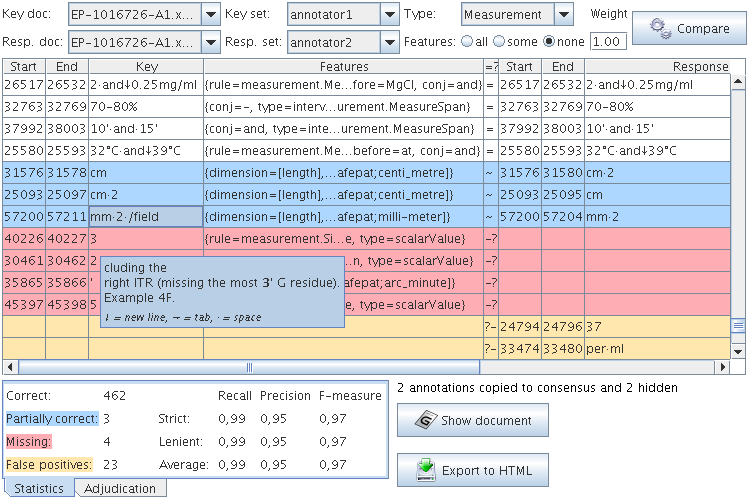
\includegraphics[width=14cm]{annotation-diff-statistics.png}
\end{center}
\caption{Annotation diff window with the parameters at the top,
the comparison table in the center and the statistics panel at the
bottom.}
\label{fig:annotdiff}
\end{figure}

The Annotation Diff tool is activated by selecting it from the Tools menu
at the top of the GATE Developer window. It will appear in a new
window.  Select the key and response documents to be used (note that
both must have been previously loaded into the system), the annotation
sets to be used for each, and the annotation type to be compared.

Note that the tool automatically intersects all the annotation
types from the selected key annotation set with all types from the
response set.

On a separate note, you can perform a diff on the same document,
between two different annotation sets. One annotation set could
contain the key type and another could contain the response one.

After the type has been selected, the user is required to decide
how the features will be compared. It is important to know that
the tool compares them by analysing if features from the key set
are contained in the response set. It checks for both the feature
name and feature value to be the same.

There are three basic options to select:
\begin{itemize}
\item
To take `all' the features from the key set into consideration
\item
To take only `some' user selected features
\item
To take `none' of the features from the key set.
\end{itemize}

The weight for the F-Measure can also be changed - by default it is set to
1.0 (i.e. to give precision and recall equal weight). Finally, click on
`Compare' to display the results. Note that the window may need to be
resized manually, by dragging the window edges as appropriate).

In the main window, the key and response annotations will be
displayed. They can be sorted by any category by clicking on the
central column header: `=?'. The key and response annotations will be
aligned if their indices are identical, and are color coded
according to the legend displayed at the bottom.

Precision, recall, F-measure are also displayed below the annotation tables,
each according to 3 criteria - strict, lenient and average. See Sections
\ref{sec:eval:annotationdiff} and \ref{sec:eval:metrics} for more
details about the evaluation metrics.

The results can be saves to an HTML file by using the `Export to
HTML' button. This creates an HTML snapshot of what the Annotation Diff
table shows at that moment. The columns and rows in the table will
be shown in the same order, and the hidden columns will not appear in
the HTML file. The colours will also be the same.

If you need more details or context you can use the button `Show document'
to display the document and the annotations selected in the annotation diff
drop down lists and table.

%%%%%%%%%%%%%%%%%%%%%%%%%%%%%%%%%%%%%%%%%%%%%%%%%%%%%%%%%%%%%%%%%%%%%%%%%%%%%
\subsect[sec:eval:adiff:goldstandard]{Creating a Gold Standard with the
Annotation Diff Tool}
%%%%%%%%%%%%%%%%%%%%%%%%%%%%%%%%%%%%%%%%%%%%%%%%%%%%%%%%%%%%%%%%%%%%%%%%%%%%%

\begin{figure}[htbp]
\begin{center}
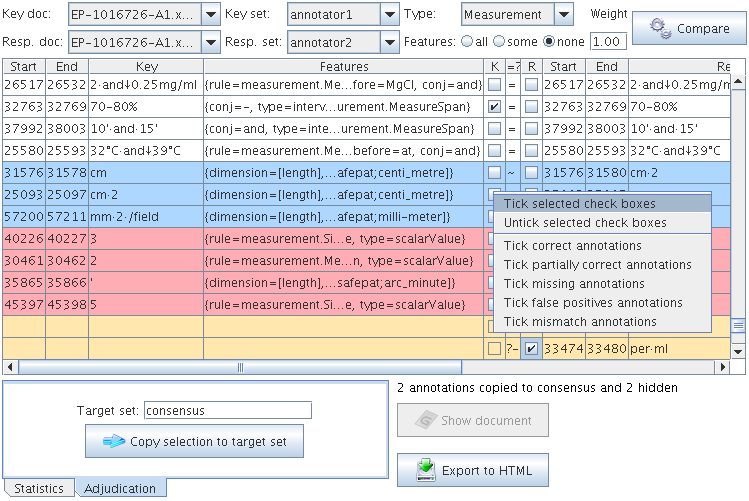
\includegraphics[width=14cm]{annotation-diff-adjudication.png}
\end{center}
\caption{Annotation diff window with the parameters at the top,
the comparison table in the center and the adjudication panel at the
bottom.}
\label{fig:annotdiff2}
\end{figure}

In order to create a gold standard set from two sets you need to show the
`Adjudication' panel at the bottom. It will insert two checkboxes columns in
the central table. Tick boxes in the columns `K(ey)' and `R(esponse)' then
input a Target set in the text field and use the `Copy selection to target'
button to copy all annotations selected to the target annotation set.

There is a context menu for the checkboxes to tick them quickly.

Each time you will copy the selection to the target set to create the gold
standard set, the rows will be hidden in further comparisons. In this way,
you will see only the annotations that haven't been processed. At the end of
the gold standard creation you should have an empty table.

To see again the copied rows, select the `Statistics' tab at the bottom and
use the button `Compare'.

%%%%%%%%%%%%%%%%%%%%%%%%%%%%%%%%%%%%%%%%%%%%%%%%%%%%%%%%%%%%%%%%%%%%%%
\sect[sec:eval:corpusqualityassurance]{Corpus Quality Assurance}
%%%%%%%%%%%%%%%%%%%%%%%%%%%%%%%%%%%%%%%%%%%%%%%%%%%%%%%%%%%%%%%%%%%%%%

\begin{figure}[htbp]
\begin{center}
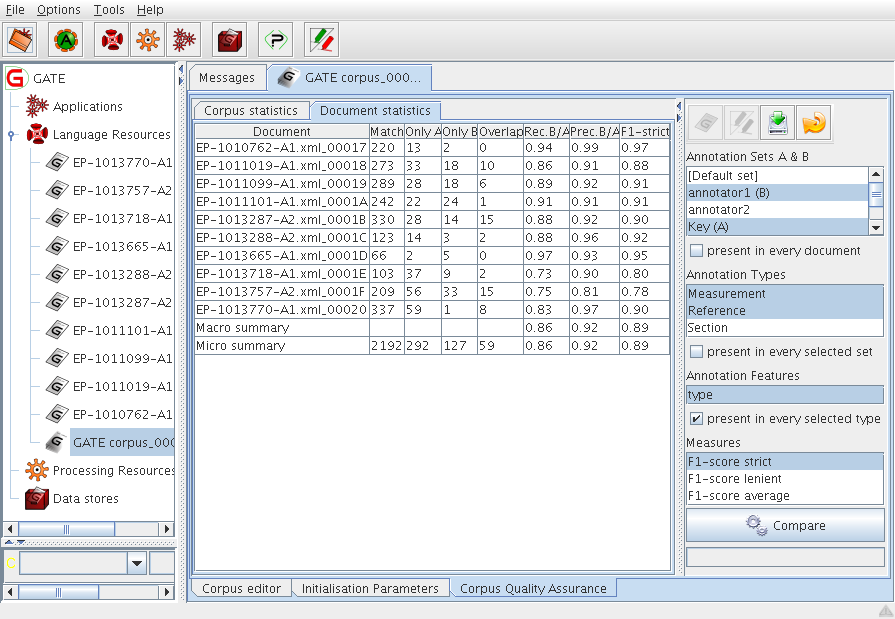
\includegraphics[width=14cm]{corpusqa.png}
\end{center}
\caption{Corpus Quality Assurance showing the document statistics table}
\label{fig:corpusqa}
\end{figure}

%%%%%%%%%%%%%%%%%%%%%%%%%%%%%%%%%%%%%%%%%%%%%%%%%%%%%%%%%%%%%%%%%%%%%%
\subsection{Description of the interface}

A bottom tab in each corpus view is entitled `Corpus Quality
Assurance'. This tab will allow you to calculate precision, recall and F-score
between two annotation sets in a corpus without the need to load a plugin. It
extends the Annotation Diff functionality to the entire corpus in a convenient
interface.

The main part of the view consists of two tabs each containing a table. One tab
is entitled `Corpus statistics' and the other is entitled `Document
statistics'.

To the right of the tabbed area is a configuration pane in which
you can select the annotation sets you wish to compare, the annotation types
you are interested in and the annotation features you wish to specify for use
in the calculation if any.

You can also choose whether to calculate agreement
on a strict or lenient basis or take the average of the two. (Recall that strict
matching requires two annotations to have an identical span if they are to be
considered a match, where lenient matching accepts a partial match; annotations
are overlapping but not identical in span.)

At the top, several icons are for opening a document (double-clicking on a
row is also working) or Annotation Diff only when a row in the document
statistics table is selected, exporting the tables to an HTML file,
reloading the list of sets, types and features when some documents have been
modified in the corpus and getting this help page.

Corpus Quality Assurance works also with a corpus inside a datastore. Using a
datastore is useful to minimise memory consumption when you have a big
corpus.

See the section~\ref{sec:eval:metrics} for more details about the evaluation
metrics.

%%%%%%%%%%%%%%%%%%%%%%%%%%%%%%%%%%%%%%%%%%%%%%%%%%%%%%%%%%%%%%%%%%%%%%
\subsection{Step by step usage}

Begin by selecting the annotation sets you wish to compare in the top list
in the configuration pane. Clicking on an annotation set labels it
annotation set A for the Key (an `(A)' will appear beside it to indicate
that this is your selection for annotation set A). Now click on another
annotation set. This will be labelled annotation set B for the response.

To change your selection, deselect an annotation set by
clicking on it a second time. You can now choose another annotation set. Note
that you do not need to hold the control key down to select the second
annotation set. This list is configured to accept two (and no more than two)
selections. If you wish, you may check the box `present in every document' to
reduce the annotation sets list to only those sets present in every document.

You may now choose the annotation types you are interested in. If you don't
choose any then all will be used. If you wish, you may check the box
`present in every selected set' to reduce the annotation types list to only
those present in every selected annotation set.

You can choose the annotation features you wish to include in the
calculation. If you choose features, then for an annotation to be considered
a match to another, their feature values must also match. If you select the
box `present in every selected type' the features list will be reduced to
only those present in every type you selected.

For the classification measures you must select only one type and one feature.

The `Measures' list allows you to choose whether to calculate strict or lenient
figures or average the two. You may choose as many as you wish, and they will
be included as columns in the table to the left. The BDM measures allow to
accept a match when the two concept are close enough in an ontology even if
their name are different. See section~\ref{sec:eval:bdmplugin}.

An `Options' button above the `Measures' list gives let you set some
settings like the beta for the Fscore or the BDM file.

Finally, click on the `Compare' button to recalculate the tables. The figures
that appear in the several tables (one per tab) are described below.

%%%%%%%%%%%%%%%%%%%%%%%%%%%%%%%%%%%%%%%%%%%%%%%%%%%%%%%%%%%%%%%%%%%%%%
\subsection{Details of the Corpus statistics table}

In this table you will see that one row appears for every annotation type
you chose. Columns give total counts for matching annotations (`Match'
equivalent to TREC Correct), annotations only present in annotation set
A/Key (`Only A' equivalent to TREC Missing), annotations only present in
annotation set B/Response (`Only B' equivalent to TREC Spurious) and
annotations that overlapped (`Overlap' equivalent to TREC Partial).

Depending on whether one of your annotation sets is considered a
gold standard, you might prefer to think of `Only A' as missing and `Only B' as
spurious, or vice versa, but the Corpus Quality Assurance tool makes no
assumptions about which if any annotation set is the gold standard. Where it is
being used to calculate Inter Annotator Agreement there is no concept of a
`correct' set. However, in `MUC' terms, `Match' would be correct and `Overlap'
would be partial.

After these columns, three columns appear for every measure
you chose to calculate. If you chose to calculate a strict F1, a recall,
precision and F1 column will appear for the strict counts. If you chose to
calculate a lenient F1, precision, recall and F1 columns will also appear for
lenient counts.

In the corpus statistics table, calculations are done on a per type
basis and include all documents in the calculation. Final rows in the table
provide summaries; total counts are given along with a micro and a macro average.

Micro averaging treats the entire corpus as one big document where macro
averaging, on this table, is the arithmetic mean of the per-type figures. See
Section~\ref{sec:eval:macromicro} for more detail on the distinction between a
micro and a macro average.

%%%%%%%%%%%%%%%%%%%%%%%%%%%%%%%%%%%%%%%%%%%%%%%%%%%%%%%%%%%%%%%%%%%%%%
\subsection{Details of the Document statistics table}

In this table you will see that one row appears for
every document in the corpus. Columns give counts as in the corpus statistics
table, but this time on a per-document basis.

As before, for every measure you
choose to calculate, precision, recall and F1 columns will appear in the table.

Summary rows, again, give a macro average (arithmetic mean of the per-document
measures) and micro average (identical to the figure in the corpus
statistics table).

%%%%%%%%%%%%%%%%%%%%%%%%%%%%%%%%%%%%%%%%%%%%%%%%%%%%%%%%%%%%%%%%%%%%%%
\subsection{GATE Embedded API for the measures}

You can get the same results as the Corpus Quality Assurance tool from your
program by using the classes that compute the results.

They are three for the moment:
\htlink{http://gate.ac.uk/gate/src/gate/util/AnnotationDiffer.java}
{AnnotationDiffer},
\htlink{http://gate.ac.uk/gate/src/gate/util/ClassificationMeasures.java}
{ClassificationMeasures} and
\htlink{http://gate.ac.uk/gate/src/gate/util/OntologyMeasures.java}
{OntologyMeasures}. All in gate.util package.

To compute the measures respect the order below.

Constructors and methods to initialise the measure objects:
\begin{small}\begin{verbatim}
AnnotationDiffer differ = new AnnotationDiffer();
differ.setSignificantFeaturesSet(Set<String> features);
ClassificationMeasures classificationMeasures = new ClassificationMeasures();
OntologyMeasures ontologyMeasures = new OntologyMeasures();
ontologyMeasures.setBdmFile(URL bdmFileUrl);
\end{verbatim}\end{small}

With bdmFileUrl an URL to a file of the format described at
section~\ref{sec:eval:bdmplugin}.

Methods for computing the measures:
\begin{small}\begin{verbatim}
differ.calculateDiff(Collection key, Collection response)
classificationMeasures.calculateConfusionMatrix(AnnotationSet key,
 AnnotationSet response, String type, String feature, boolean verbose)
ontologyMeasures.calculateBdm(Collection<AnnotationDiffer> differs)
\end{verbatim}\end{small}

With verbose to be set to true if you want to get printed the annotations
ignored on the "standard" output stream.

Constructors, useful for micro average, no need to use calculateX methods
as they must have been already called:
\begin{small}\begin{verbatim}
AnnotationDiffer(Collection<AnnotationDiffer> differs)
ClassificationMeasures(Collection<ClassificationMeasures> tables)
OntologyMeasures(Collection<OntologyMeasures> measures)
\end{verbatim}\end{small}

Method for getting results for all 3 classes:
\begin{small}\begin{verbatim}
List<String> getMeasuresRow(Object[] measures, String title)
\end{verbatim}\end{small}

With measures an array of String with values to choose from:
\begin{itemize}
\item F1.0-score strict
\item F1.0-score lenient
\item F1.0-score average
\item F1.0-score strict BDM
\item F1.0-score lenient BDM
\item F1.0-score average BDM
\item Observed agreement
\item Cohen's Kappa
\item Pi's Kappa
\end{itemize}

Note that the numeric value `1.0' represents the beta coefficient in the Fscore.
See section~\ref{sec:eval:metrics} for more information on these measures.

Method only for ClassificationMeasures:
\begin{small}\begin{verbatim}
List<List<String>> getConfusionMatrix(String title)
\end{verbatim}\end{small}

The following example is taken from
\htlink{http://gate.ac.uk/gate/src/gate/gui/CorpusQualityAssurance.java}
{gate.gui.CorpusQualityAssurance\#compareAnnotation} but hasn't been ran so
there could be some corrections to make.

\begin{lstlisting}
  final int FSCORE_MEASURES = 0;
  final int CLASSIFICATION_MEASURES = 1;
  ArrayList<String> documentNames = new ArrayList<String>();
  TreeSet<String> types = new TreeSet<String>();
  Set<String> features = new HashSet<String>();

  int measuresType = FSCORE_MEASURES;
  Object[] measures = new Object[]
    {"F1.0-score strict", "F0.5-score lenient BDM"};
  String keySetName = "Key";
  String responseSetName = "Response";
  types.add("Person");
  features.add("gender");
  URL bdmFileUrl = null;
  try {
    bdmFileUrl = new URL("file:///tmp/bdm.txt");
  } catch (MalformedURLException e) {
    e.printStackTrace();
  }

  boolean useBdm = false;
  for (Object measure : measures) {
    if (((String) measure).contains("BDM")) { useBdm = true; break; }
  }

  // for each document
  for (int row = 0; row < corpus.size(); row++) {
    boolean documentWasLoaded = corpus.isDocumentLoaded(row);
    Document document = (Document) corpus.get(row);
    documentNames.add(document.getName());
    Set<Annotation> keys = new HashSet<Annotation>();
    Set<Annotation> responses = new HashSet<Annotation>();
    // get annotations from selected annotation sets
    keys = document.getAnnotations(keySetName);
    responses = document.getAnnotations(responseSetName);
    if (!documentWasLoaded) { // in case of datastore
      corpus.unloadDocument(document);
      Factory.deleteResource(document);
    }

    // fscore document table
    if (measuresType == FSCORE_MEASURES) {
      HashMap<String, AnnotationDiffer> differsByType =
        new HashMap<String, AnnotationDiffer>();
      AnnotationDiffer differ;
      Set<Annotation> keysIter = new HashSet<Annotation>();
      Set<Annotation> responsesIter = new HashSet<Annotation>();
      for (String type : types) {
        if (!keys.isEmpty() && !types.isEmpty()) {
          keysIter = ((AnnotationSet)keys).get(type);
        }
        if (!responses.isEmpty() && !types.isEmpty()) {
          responsesIter = ((AnnotationSet)responses).get(type);
        }
        differ = new AnnotationDiffer();
        differ.setSignificantFeaturesSet(features);
        differ.calculateDiff(keysIter, responsesIter); // compare
        differsByType.put(type, differ);
      }
      differsByDocThenType.add(differsByType);
      differ = new AnnotationDiffer(differsByType.values());
      List<String> measuresRow;
      if (useBdm) {
        OntologyMeasures ontologyMeasures = new OntologyMeasures();
        ontologyMeasures.setBdmFile(bdmFileUrl);
        ontologyMeasures.calculateBdm(differsByType.values());
        measuresRow = ontologyMeasures.getMeasuresRow(
          measures, documentNames.get(documentNames.size()-1));
      } else {
        measuresRow = differ.getMeasuresRow(measures,
          documentNames.get(documentNames.size()-1));
      }
      System.out.println(Arrays.deepToString(measuresRow.toArray()));

    // classification document table
    } else if (measuresType == CLASSIFICATION_MEASURES
           && !keys.isEmpty() && !responses.isEmpty()) {
      ClassificationMeasures classificationMeasures =
        new ClassificationMeasures();
      classificationMeasures.calculateConfusionMatrix(
        (AnnotationSet) keys, (AnnotationSet) responses,
        types.first(), features.iterator().next(), false);
      List<String> measuresRow = classificationMeasures.getMeasuresRow(
        measures, documentNames.get(documentNames.size()-1));
      System.out.println(Arrays.deepToString(measuresRow.toArray()));
      List<List<String>> matrix = classificationMeasures
        .getConfusionMatrix(documentNames.get(documentNames.size()-1));
      for (List<String> matrixRow : matrix) {
        System.out.println(Arrays.deepToString(matrixRow.toArray()));
      }
    }
  }
\end{lstlisting}

See method
\htlink{http://gate.ac.uk/gate/src/gate/gui/CorpusQualityAssurance.java}
{gate.gui.CorpusQualityAssurance\#printSummary} for micro and macro average
like in the Corpus Quality Assurance.

%%%%%%%%%%%%%%%%%%%%%%%%%%%%%%%%%%%%%%%%%%%%%%%%%%%%%%%%%%%%%%%%%%%%%%
\subsection[sec:eval:qapr]{Quality Assurance PR}

We have also implemented a processing resource called Quality Assurance PR that
wraps the functionality of the QA Tool.  At the time of writing this 
documentation, the only difference the QA PR has in terms of functionality is 
that the PR only accepts one measure at a time.

The Quality Assuarance PR is included in the Tools plugin.  The PR can be added 
to any existing corpus pipeline.  Since the QA tool works on the entire corpus, 
the PR has to be executed after all the documents in the corpus have been 
processed.  In order to achieve this, we have designed the PR in such a way that
it only gets executed when the pipeline reaches to the last document in the 
corpus.  There are no init-time parameters but users are required to provide 
values for the following run-time parameters.

\begin{itemize}
\item annotationTypes - annotation types to compare.
\item featuresNames - features of the annotation types (specified above) to 
compare.
\item keyASName - the annotation set that acts as a gold standard set and 
contains annotations of the types specified above in the first parameter.
\item responseASName - the annotation set that acts as a test set and contains 
annotations of the types specified above in the first parameter.
\item measure - one of the six pre-defined measures: F1\_STRICT, F1\_AVERAGE,
F1\_LENIENT, F05\_STRICT, F05\_AVERAGE and F05\_LENIENT.
\item outputFolderUrl - the PR produces two html files in the folder mentioned 
in this parameter.  The files are document-stats.html and the corpus-stats.html.
The former lists statistics for each document and the latter lists statistics 
for each annotation type in the corpus. In case of the document-stats.html, each
document is linked with an html file that contains the output of the
annotation diff utility in GATE.
\end{itemize}

%%%%%%%%%%%%%%%%%%%%%%%%%%%%%%%%%%%%%%%%%%%%%%%%%%%%%%%%%%%%%%%%%%%%%%
\sect[sec:eval:benchmarktool]{Corpus Benchmark Tool}
%%%%%%%%%%%%%%%%%%%%%%%%%%%%%%%%%%%%%%%%%%%%%%%%%%%%%%%%%%%%%%%%%%%%%%

Like the Corpus Quality Assurance functionality, the corpus benchmark tool
 enables evaluation to be carried out over a whole corpus rather than a
single document. Unlike Corpus QA, it uses matched corpora to achieve this,
rather than comparing annotation sets within a corpus. It enables tracking of the
system's performance over time. It provides more detailed information regarding
the annotations that differ between versions of the corpus (e.g. annotations
created by different versions of an application) than the Corpus QA tool does.
% The tool can be run either from GATE Developer or the command line.

The basic idea with the tool is to evaluate an application with respect to a
`gold standard'. You have a `marked' corpus containing the gold standard
reference annotations; you have a `clean' copy of the corpus that does not
contain the annotations in question, and you have an application that creates the
annotations in question. Now you can see how you are getting on, by comparing the
result of running your application on `clean' to the `marked' annotations.

%%%%%%%%%%%%%%%%%%%%%%%%%%%%%%%%%%%%%%%%%%%%%%%%%%%%%%%%%%%%%%%%%%%%%%%%%%%%%
\subsect[sec:eval:preparing-benchmarktool]{Preparing the Corpora for Use}
%%%%%%%%%%%%%%%%%%%%%%%%%%%%%%%%%%%%%%%%%%%%%%%%%%%%%%%%%%%%%%%%%%%%%%%%%%%%%

You will need to prepare the following directory structure:

\begin{small}\begin{verbatim}
main directory (can have any name)
|
|__"clean" (directory containing unannotated documents in XML form)
|
|__"marked" (directory containing annotated documents in XML form)
|
|__"processed" (directory containing the datastore which is generated
               when you `store corpus for future evaluation')
\end{verbatim}\end{small}

\begin{itemize}
  
\item {\bf main}: you should have a main directory containing subdirectories for
  your matched corpora. It does not matter what this directory is called. This
  is the directory you will select when the program prompts, `Please select a
  directory which contains the documents to be evaluated'.

\item {\bf clean}: Make a directory called `clean' (case-sensitive), and in it,
make a copy of your corpus that does not contain the annotations that your
application creates (though it may contain other annotations). The corpus
benchmark tool will apply your application to this corpus, so it is important
that the annotations it creates are not already present in the corpus. You can
create this corpus by copying your `marked' corpus and deleting the annotations
in question from it.

\item {\bf marked}: you should have a `gold standard' copy of your corpus in a
directory called `marked' (case-sensitive), containing the annotations to which
the program will compare those produced by your application. The idea of the
corpus benchmark tool is to tell you how good your application performance is relative
to this annotation set. The `marked' corpus should contain exactly the same
documents as the `clean' set.

\item {\bf processed}: this directory contains a third version of the corpus.
This directory will be created by the tool itself, when you run `store corpus for
future evaluation'. We will explain how to do this in
Section~\ref{sec:eval:howto-benchmarktool}

\end{itemize}

%%%%%%%%%%%%%%%%%%%%%%%%%%%%%%%%%%%%%%%%%%%%%%%%%%%%%%%%%%%%%%%%%%%%%%%%%%%%%
\subsect[sec:eval:corpustoolproperties]{Defining Properties}
%%%%%%%%%%%%%%%%%%%%%%%%%%%%%%%%%%%%%%%%%%%%%%%%%%%%%%%%%%%%%%%%%%%%%%%%%%%%%

The properties of the corpus benchmark tool are defined in the file
`corpus\_tool.properties', which should be located in the GATE home directory. GATE
will tell you where it's looking for the properties file in the `message' panel
when you run the Corpus Benchmark Tool. It is important to prepare this file
before attempting to run the tool because there is no file present by default, so
unless you prepare this file, the corpus benchmark tool will not work!

The following properties should be set:
\begin{itemize}
\item the precision/recall performance threshold for verbose mode, below which
the annotation will be displayed in the results file. This enables problem
annotations to be easily identified. By default this is set to 0.5;
\item the name of the annotation set containing the human-marked
annotations (annotSetName);
\item the name of the annotation set containing the system-generated
annotations (outputSetName);
\item the annotation types to be considered (annotTypes);
\item the feature values to be considered, if any (annotFeatures).
\end{itemize}

The default annotation set has to be represented by an empty string. The
outputSetName and annotSetName must be different, and cannot both be the default
annotation set. (If they are the same, then use the Annotation Set Transfer PR to
change one of them.) If you omit any line (or just leave the value blank), that
property reverts to default. For example, `annotSetName=' is the same as leaving
that line out.

An example file is shown below:
\begin{small}\begin{verbatim}
threshold=0.7
annotSetName=Key
outputSetName=ANNIE
annotTypes=Person;Organization;Location;Date;Address;Money
annotFeatures=type;gender
\end{verbatim}\end{small}

Here is another example:
\begin{small}\begin{verbatim}
threshold=0.6  
annotSetName=Filtered  
outputSetName=  
annotTypes=Mention  
annotFeatures=class  
\end{verbatim}\end{small}

%%%%%%%%%%%%%%%%%%%%%%%%%%%%%%%%%%%%%%%%%%%%%%%%%%%%%%%%%%%%%%%%%%%%%%%%%%%%%
\subsect[sec:eval:howto-benchmarktool]{Running the Tool}
%%%%%%%%%%%%%%%%%%%%%%%%%%%%%%%%%%%%%%%%%%%%%%%%%%%%%%%%%%%%%%%%%%%%%%%%%%%%%

To use the tool, first make sure the properties of the tool have been set
correctly (see Section \ref{sec:eval:corpustoolproperties} for how to do this)
and that the corpora and directory structure have been prepared as outlined in
Section~\ref{sec:eval:preparing-benchmarktool}. Also, make sure that your
application is {\bf saved to file} (see Section~\ref{sec:developer:savestate}).
Then, from the `Tools' menu, select `Corpus Benchmark'. You have four options:

\begin{enumerate}
  \item Default Mode
  \item Store Corpus for Future Evaluation
  \item Human Marked Against Stored Processing Results
  \item Human Marked Against Current Processing Results
\end{enumerate}

We will describe these options in a different order to that in which they
appear on the menu, to facilitate explanation.

{\bf Store Corpus for Future Evaluation} populates the `processed' directory with
a datastore containing the result of running your application on the `clean'
corpus. If a `processed' directory exists, the results will be placed there; if
not, one will be created. This creates a record of the current application
performance. You can rerun this operation any time to update the stored set.

{\bf Human Marked Against Stored Processing Results} compares the stored
`processed' set with the `marked' set. This mode assumes you have already run
`Store corpus for future evaluation'. It performs a diff between the `marked'
directory and the `processed' directory and prints out the metrics.

{\bf Human Marked Against Current Processing Results} compares the `marked' set
with the result of running the application on the `clean' corpus. It runs your
application on the documents in the `clean' directory creating a temporary
annotated corpus and performs a diff with the documents in the `marked'
directory. After the metrics (recall, precision, etc.) are calculated and printed
out, it deletes the temporary corpus.

{\bf Default Mode} runs `Human Marked Against Current Processing Results' and
`Human Marked Against Stored Processing Results' and compares the results of the
two, showing you where things have changed between versions. This is one of the
main purposes of the benchmark tool; to show the difference in performance
between different versions of your application.

Once the mode has been selected, the program prompts, `Please select a directory
which contains the documents to be evaluated'. Choose the main directory
containing your corpus directories. (Do not select `clean', `marked', or
`processed'.) Then (except in `Human marked against stored processing
results' mode) you will be prompted to select the file containing your
application (e.g. an .xgapp file).

The tool can be used either in verbose or non-verbose mode, by selecting or
unselecting the verbose option from the menu. In verbose mode, for any
precision/recall figure below the user's pre-defined threshold (stored in
corpus\_tool.properties file) the tool will show the the non-coextensive
annotations (and their corresponding text) for that entity type, thereby enabling
the user to see where problems are occurring.

%%%%%%%%%%%%%%%%%%%%%%%%%%%%%%%%%%%%%%%%%%%%%%%%%%%%%%%%%%%%%%%%%%%%%%%%%%%%%
\subsect[sec:eval:results-benchmarktool]{The Results}
%%%%%%%%%%%%%%%%%%%%%%%%%%%%%%%%%%%%%%%%%%%%%%%%%%%%%%%%%%%%%%%%%%%%%%%%%%%%%

Running the tool (either in `Human marked against stored processing results',
`Human marked against current processing results' or `Default' mode) produces an
HTML file, in tabular form, which is output in the main GATE Developer messages
window. This can then be pasted into a text editor and viewed in a web
browser for easier viewing. See figure \ref{fig:benchmark} for an example.

In each mode, the following statistics will be output:

\begin{enumerate}
  \item Per-document figures, itemised by type: precision and recall, as well as
  detailed information about the differing annotations;
  \item Summary by type (`Statistics'): correct, partially correct, missing
  and spurious totals, as well as whole corpus (micro-average) precision,
  recall and f-measure (F1), itemised by type;
  \item Overall average figures: precision, recall and F1 calculated as a
  macro-average (arithmetic average) of the individual document precisions and recalls.
\end{enumerate}

In `Default' mode, information is also provided about whether the figures have
increased or decreased in comparison with the `Marked' corpus.

\begin{figure}[htbp]
\begin{center}
\fbox{
 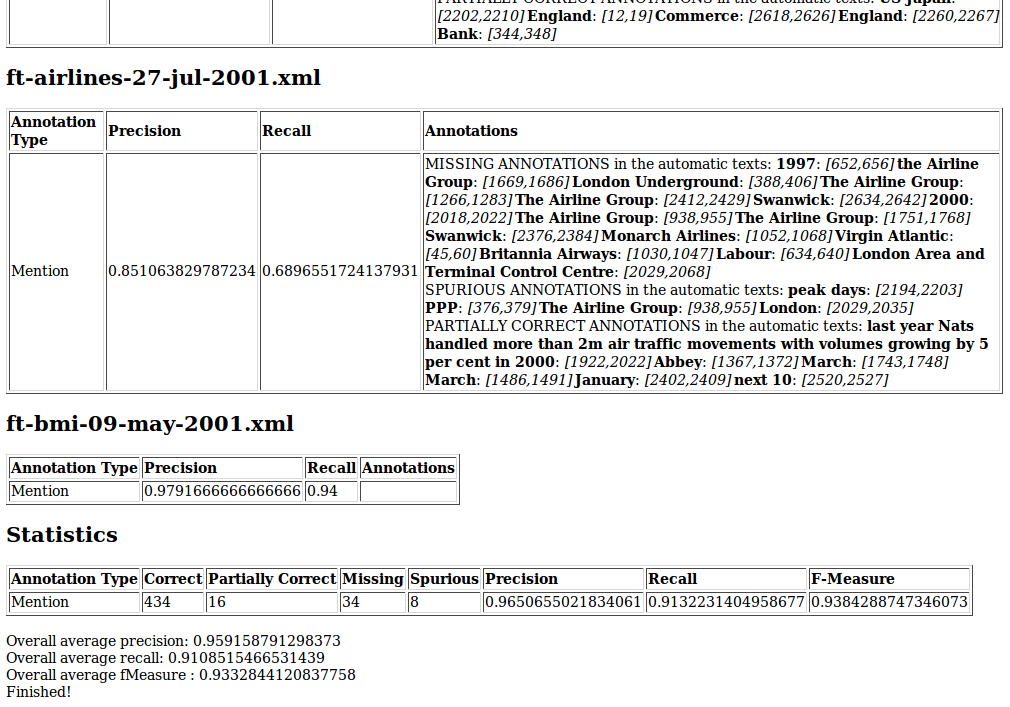
\includegraphics[width=14cm]{cbt.png}
}
\end{center}
\caption{Fragment of results from corpus benchmark tool}
\label{fig:benchmark}
\end{figure}

%The Corpus Benchmark tool can be run in two ways: standalone and GUI mode.
%Section \ref{sec:gui:benchmarktool} describes the theory behind this tool.
%
%\subsect{GUI mode}


%\subsect{Standalone mode}

%Alternatively, the tool can be run in standalone mode, using the
%following commands:
%
%\begin{itemize}
%
%\item To process the corpus, issue the command
%\begin{small}\begin{verbatim}gate -e -generate corpusname \end{verbatim}\end{small}
%(where 'corpusname' is the name of the corpus)
%
%\item To run in Stored mode, issue the command
%\begin{small}\begin{verbatim}gate -e [-verbose] -marked\_stored corpusname \end{verbatim}\end{small}
%
%\item To run in Current mode, issue the command
%\begin{small}\begin{verbatim}gate -e [-verbose] -marked\_clean corpusname \end{verbatim}\end{small}
%
%\item To run in Default mode, issue the command
%\begin{small}\begin{verbatim}gate -e [-verbose] corpusname \end{verbatim}\end{small}
%
%\end{itemize}
%The tool can be run in verbose mode for any of these options using the
% [-verbose] flag. The results can be piped to an html
% file and viewed with an internet browser.

%%%%%%%%%%%%%%%%%%%%%%%%%%%%%%%%%%%%%%%%%%%%%%%%%%%%%%%%%%%%%%%%%%%%%%%%%%%%%
\sect[sec:eval:iaaplugin]{A Plugin Computing Inter-Annotator Agreement (IAA)}
%%%%%%%%%%%%%%%%%%%%%%%%%%%%%%%%%%%%%%%%%%%%%%%%%%%%%%%%%%%%%%%%%%%%%%%%%%%%%

The interannotator agreement plugin, `Inter\_Annotator\_Agreement', computes the
F-measures, namely precision, recall and F1, suitable for named entity
annotations (see Section~\ref{sec:eval:prf}), and agreement, Cohen's kappa and
Scott's pi, suitable for text classification tasks (see
Section~\ref{sec:eval:kappa}). In the latter case, a confusion matrix is also
provided. In this section we describe those measures and the output results from
the plugin. But first we explain how to load the plugin, and the input to and the
parameters of the plugin.

First you need to load the plugin named `Inter\_Annotator\_Agreement' into
GATE Developer using the tool {\em Manage CREOLE Plugins}, if it is not
already loaded.  Then you can create a PR for the plugin from the
`IAA Computation' in the existing PR list. After that you can put
the PR into a {\em Corpus Pipeline} to use it.

The IAA Computation PR differs from the Corpus Benchmark Tool in the data
preparation required. As in the Corpus Benchmark Tool, the idea is to compare
annotation sets, for example, prepared by different annotators, but in the IAA
Computation PR, these annotation sets should be on the same set of documents.
Thus, one corpus is loaded into GATE on which the PR is run. Different annotation
sets contain the annotations which will be compared. These should (obviously)
have different names.

It falls to the user to decide whether to use annotation type or an annotation
feature as class; are two annotations considered to be in agreement because they
have the same type and the same span? Or do you want to mark up your data with an
annotation type such as `Mention', thus defining the relevant annotations, then
give it a `class' feature, the value of which should be matched in order that
they are considered to agree? This is a matter of convenience. For example, data
from the Batch Learning PR (see Section~\ref {sec:ml:batch-learning-pr}) uses a
single annotation type and a class feature. In other contexts, using annotation
type might feel more natural; the annotation sets should agree about what is a
`Person', what is a `Date' etc. It is also possible to mix the two, as you will
see below.

The IAA plugin has two runtime parameters {\bf annSetsForIaa} and {\bf
annTypesAndFeats} for specifying the annotation sets and the annotation types and
features, respectively. Values should be separated by semicolons. For example, to
specify annotation sets `Ann1', `Ann2' and `Ann3' you should set the value of
{\em annSetsForIaa} to `Ann1;Ann2;Ann3'. Note that more than two annotation sets
are possible. Specify the value of {\em annTypesAndFeats} as `Per' to compute the
IAA for the three annotation sets on the annotation type {\em Per}. You can also
specify more than one annotation type and separate them by `;' too, and
optionally specify an annotation feature for a type by attaching a `-$>$'
followed by feature name to the end of the annotation name.  For example,
`Per-$>$label;Org' specifies two annotation types {\em Per} and {\em Org} and
also a feature name {\em label} for the type {\em Per}. If you specify an
annotation feature for an annotation type, then two annotations of the same type
will be regarded as being different if they have different values of that
feature, even if the two annotations occupy exactly the same position in the
document. On the other hand, if you do not specify any annotation feature for an
annotation type, then the two annotations of the type will be regarded as the
same if they occupy the same position in the document.

The parameter {\bf measureType} specifies the type of measure computed. There are
two measure types; the {\em F-measure} (i.e. Precision, Recall and F1), and the
{\em observed agreement and Cohen's Kappa}.  For classification tasks such as
document or sentence classification, the observed agreement and Cohen's Kappa is
often used, though the F-measure is applicable too. In these tasks, the targets
are already identified, and the task is merely to classify them correctly.
However, for the named entity recognition task, only the F-measure is applicable.
In such tasks, finding the `named entities' (text to be annotated) is as much a
part of the task as correctly labelling it. Observed agreement and Cohen's kappa
are not suitable in this case. See Section~\ref{sec:eval:kappa} for further
discussion. The parameter has two values, {\em FMEASURE} and {\em
AGREEMENTANDKAPPA}. The default value of the parameter is {\em FMEASURE}.

Another parameter {\bf verbosity} specifies the verbosity level of the
plugin's output. Level 2 displays the most detailed output, including
the IAA measures on each document and the macro-averaged results over
all documents.  Level 1 only displays the IAA measures averaged over
all documents.  Level 0 does not have any output. The default value of
the parameter is 1.  In the following we will explain the outputs in
detail.

Yet another runtime parameter {\bf bdmScoreFile} specifies the URL for
a file containing the BDM scores used for the BDM based IAA
computation. The BDM score file should be produced by the BDM
computation plugin, which is described in
Section \ref{sec:eval:bdmplugin}. The BDM-based IAA computation will be
explained below.  If the parameter is not assigned any value, or is
assigned a file which is not a BDM score file, the PR will not compute the
BDM based IAA.

%%%%%%%%%%%%%%%%%%%%%%%%%%%%%%%%%%%%%%%%%%%%%%%%%%%%%%%%%%%%%%%%%%%%%%%%%%%%%
\subsection{IAA for Classification}
%%%%%%%%%%%%%%%%%%%%%%%%%%%%%%%%%%%%%%%%%%%%%%%%%%%%%%%%%%%%%%%%%%%%%%%%%%%%%

IAA has been used mainly in classification tasks, where two or more annotators
are given a set of instances and are asked to classify those instances into some
pre-defined categories. IAA measures the agreements among the annotators on the
class labels assigned to the instances by the annotators. Text classification
tasks include document classification, sentence classification (e.g. opinionated
sentence recognition), and token classification (e.g. POS tagging). The important
point to note is that the evaluation set and gold standard set have exactly the
same instances, but some instances in the two sets have different class labels.
Identifying the instances is not part of the problem.

The three commonly used IAA measures are {\em observed agreement}, {\em specific
agreement}, and {\em Kappa ($\kappa$)} \cite{Hripcsak02}. See
Section~\ref{sec:eval:kappa} for the detailed explanations of those measures. If
you select the value of the runtime parameter {\em measureType} as {\em
AGREEMENTANDKAPPA}, the IAA plugin will compute and display those IAA measures
for your classification task. Below, we will explain the output of the
PR for the agreement and Kappa measures.

At the verbosity level 2, the output of the plugin is the most detailed. It first
prints out a list of the names of the annotation sets used for IAA computation.
In the rest of the results, the first annotation set is denoted as annotator
0, and the second annotation set is denoted as annotator 1, etc.  Then the plugin
outputs the IAA results for each document in the corpus.

For each document, it displays one annotation type and optionally an annotation
feature if specified, and then the results for that type and that feature. Note
that the IAA computations are based on the pairwise comparison of annotators. In
other words, we compute the IAA for each pair of annotators. The first results
for one document and one annotation type are the macro-averaged ones over all
pairs of annotators, which have three numbers for the three types of IAA
measures, namely {\em Observed agreement}, {\em Cohen's kappa} and {\em Scott's
pi}. Then for each pair of annotators, it outputs the three types of measures, a
confusion matrix (or contingency table), and the specific agreements for each
label.  The labels are obtained from the annotations of that particular type. For
each annotation type, if a feature is specified, then the labels are the values
of that feature. Please note that two terms may be added to the label list: one
is the empty one obtained from those annotations which have the annotation
feature but do not have a value for the feature; the other is `Non-cat',
corresponding to those annotations not having the feature at all. If no feature
is specified, then two labels are used: `Anns' corresponding to the annotations
of that type, and `Non-cat' corresponding to those annotations which are
annotated by one annotator but are not annotated by another annotator.

After displaying the results for each document, the plugin prints out the
macro-averaged results over all documents. First, for each annotation type, it
prints out the results for each pair of annotators, and the macro-averaged
results over all pairs of annotators. Finally it prints out the macro-averaged
results over all pairs of annotators, all types and all documents.

Please note that the classification problem can be evaluated using the F-measure
too. If you want to evaluate a classification problem using the F-measure, you
just need to set the run time parameter {\em measureType} to {\em FMEASURE}.

%%%%%%%%%%%%%%%%%%%%%%%%%%%%%%%%%%%%%%%%%%%%%%%%%%%%%%%%%%%%%%%%%%%%%%%%%%%%%
\subsection{IAA For Named Entity Annotation}
%%%%%%%%%%%%%%%%%%%%%%%%%%%%%%%%%%%%%%%%%%%%%%%%%%%%%%%%%%%%%%%%%%%%%%%%%%%%%

The commonly used IAA measures, such as kappa, have not been used in text mark-up
tasks such as named entity recognition and information extraction, for reasons
explained in Section \ref{sec:eval:kappa} (also see \cite{Hripcsak05}). Instead,
the F-measures, such as Precision, Recall, and F1, have been widely used in
information extraction evaluations such as MUC, ACE and TERN for measuring IAA.
This is because the computation of the F-measures does not need to know the
number of non-entity examples. Another reason is that F-measures are commonly
used for evaluating information extraction systems. Hence IAA F-measures can be
directly compared with results from other systems published in the literature.

For computing F-measure between two annotation sets, one can use one annotation
set as gold standard and another set as system's output and compute the
F-measures such as Precision, Recall and F1. One can switch the roles of the two
annotation sets. The Precision and Recall in the former case become Recall and
Precision in the latter, respectively.  But the F1 remains the same in both
cases.  For more than two annotators, we first compute F-measures between any two
annotators and use the mean of the pair-wise F-measures as an overall measure.

The computation of the F-measures (e.g. Precision, Recall and F1) are
 shown in Section \ref{sec:eval:metrics}. As noted in \cite{Hripcsak05}, the F1
 computed for two annotators for one specific category is equivalent to the
 positive specific agreement of the category.

The outputs of the IAA plugins for named entity annotation are similar to those
for classification. But the outputs are the F-measures, such as Precision, Recall
and F1, instead of the agreements and Kappas. It first prints out the results for
each document. For one document, it prints out the results for each annotation
type, macro-averaged over all pairs of annotators, then the results for each pair
of annotators.  In the last part, the micro-averaged results over all documents
are displayed.  Note that the results are reported in both the strict measure and
the lenient measure, as defined in Section \ref{sec:eval:annotationdiff}.

Please note that, for computing the F-measures for the named entity annotations,
the IAA plugin carries out the same computation as the {\em Corpus Benchmark
tool}.  The IAA plugin is simpler than the Corpus benchmark tool in the sense
that the former needs only one set of documents with two or more annotation sets,
whereas the latter needs three sets of the same documents, one without any
annotation, another with one annotation set, and the third one with another
annotation set. Additionally, the IAA plugin can deal with more than two
annotation sets but the Corpus benchmark tool can only deal with two annotation
sets.

%%%%%%%%%%%%%%%%%%%%%%%%%%%%%%%%%%%%%%%%%%%%%%%%%%%%%%%%%%%%%%%%%%%%%%%%%%%%%
\subsection{The BDM-Based IAA Scores}
%%%%%%%%%%%%%%%%%%%%%%%%%%%%%%%%%%%%%%%%%%%%%%%%%%%%%%%%%%%%%%%%%%%%%%%%%%%%%

For a named entity recognition system, if the named entity's class
labels are the names of concepts in some ontology (e.g. in the
ontology-based information extraction), the system can be evaluated
using the IAA measures based on the BDM scores. The BDM measures the
closeness of two concepts in an ontology. If an entity is identified
but is assigned a label which is close to but not the same as the true
label, the system should obtain some credit for it, which the
BDM-based metric can do. In contrast, the conventional named entity
recognition measure does not take into account the closeness of two
labels and does not give any credit to one identified entity with a
wrong label, regardless of how close the assigned label is to the true
label. For more explanation about BDM see
Section \ref{sec:eval:bdmplugin}.

In order to compute the BDM-based IAA, one has to assign the plugin's
runtime parameter {\bf bdmScoreFile} to the URL of a file containing
the BDM scores.  The file should be obtained by using the BDM
computation plugin, which is described in
Section \ref{sec:eval:bdmplugin}. Currently the BDM-based IAA is only
used for computing the F-measures for e.g. the entity recognition
problem. Please note that the F-measures can also be used for
evaluation of classification problem.  The BDM is not used for
computing other measures such as the {\em observed agreement} and {\em
Kappa}, though it is possible to implement it.  Therefore currently
one has to select {\em FMEASURE} for the run time parameter {\em
measureType} in order to use the BDM based IAA computation.


%%%%%%%%%%%%%%%%%%%%%%%%%%%%%%%%%%%%%%%%%%%%%%%%%%%%%%%%%%%%%%%%%%%%%%%%%%%%%
\sect[sec:eval:bdmplugin]{A Plugin Computing the BDM Scores for an Ontology}
%%%%%%%%%%%%%%%%%%%%%%%%%%%%%%%%%%%%%%%%%%%%%%%%%%%%%%%%%%%%%%%%%%%%%%%%%%%%%

The BDM (balanced distance metric) measures the closeness of two
concepts in an ontology or taxonomy \cite{Maynard05a,Maynard06a}. It
is a real number between 0 and 1. The closer the two concepts are in
an ontology, the greater their BDM score is.  For detailed explanation
about the BDM, see the papers \cite{Maynard05a,Maynard06a}.  The BDM
can be seen as an improved version of the learning
accuracy \cite{Cim03b}.  It is dependent on the length of the shortest
path connecting the two concepts and also the deepness of the two
concepts in ontology. It is also normalised with the size of ontology
and also takes into account the concept density of the area containing
the two involved concepts.

The BDM has been used to evaluate the ontology based information
extraction (qOBIE) system \cite{Maynard06a}. The OBIE identifies the
instances for the concepts of an ontology. It's possible that an OBIE
system identifies an instance successfully but does not assign it the
correct concept. Instead it assigns the instance a concept being close
to the correct one.  For example, the entity `London' is an instance
of the concept {\em Capital}, and an OBIE system assigns it the
concept {\em City} which is close to the concept {\em Capital} in some
ontology.  In that case the OBIE should obtain some credit according
to the closeness of the two concepts.  That is where the BDM can be
used. The BDM has also been used to evaluate the hierarchical
classification system \cite{Yaoyong07a}. It can also be used for
ontology learning and alignment.

The BDM computation plugin computes BDM score for each pair of concepts in an
ontology.  It has two run time parameters:
\begin{itemize}
\item {\bf ontology} -- its value should the ontology that one wants to
compute the BDM scores for.
\item {\bf outputBDMFile} -- its value is the URL of a file which will store the BDM scores
computed.
\end{itemize}
The plugin has the name {\em Ontology\_BDM\_Computation} and the corresponding
processing resource's name is {\em BDM Computation PR}. The PR can be
put into a Pipeline. If it is put into a Corpus Pipeline, the corpus
used should contain at least one document.

The BDM computation used the formula given in \cite{Maynard06a}.  The
 resulting file specified by the runtime parameter {\em outputBDMFile}
 contains the BDM scores. It is a text file. The first line of the
 file gives some meta information such as the name of ontology used
 for BDM computation. From the second line of the file, each line
 corresponds to one pair of concepts. One line is like

{\em key=Service, response=Object, bdm=0.6617647, msca=Object, cp=1,
dpk=1, dpr=0, n0=2.0, n1=2.0, n2=2.8333333, bran=1.9565217}

It first shows the names of the two concepts (one as {\em key} and
another as {\em response}, and the BDM score, and then other
parameters' values used for the computation.  Note that, since the BDM
is symmetric for the two concepts, the resulting file contains only
one line for each pair. So if you want to look for the BDM score for
one pair of concepts, you can choose one as key and another as
response. If you cannot find the line for the pair, you have to change
the order of two concepts and retrieve the file again.

%%%%%%%%%%%%%%%%%%%%%%%%%%%%%%%%%%%%%%%%%%%%%%%%%%%%%%%%%%%%%%%%%%%%%%
\sect[sec:eval:qaForTW]{Quality Assurance Summariser for Teamware}

When documents are annotated using Teamware, anonymous annotation sets are 
created for the annotating annotators. This makes it impossible to run Quality 
Assurance on such documents as annotation sets with same names in different 
documents may refer to the annoations created by different annotators. This is 
specially the case when a requirement is to compute Inter Annotator Agreement 
(IAA). The \textbf{QA Summariser for Teamware} PR generates a summary of 
agreements among annotators. It does this by pairing individual annotators 
involved in the annotation task. It also compares annotations of each individual
annotator with those available in the consensus annotation set in the respective
documents.

The PR is available from the \textbf{Teamware\_Tools} plugin, but the
\textbf{Tools} plugin must be loaded before the \textbf{Teamware\_Tools} one
because the QA summariser PR internally uses the QualityAssurancePR (from
\textbf{Tools}) to calculate agreement statistics.  User has to provide the
following run-time parameters:

\begin{itemize}
\item \textbf{annotationTypes}  Annotation types for which the IAA has to be 
  computed.
\item \textbf{featureNames}  Features of annotations that should be used in IAA 
  computations. If no value is provided, only annotation boundaries for same
  annotation types are compared.
\item \textbf{measure}
  one of the six pre-defined measures: F1\_STRICT, F1\_AVERAGE,
F1\_LENIENT, F05\_STRICT, F05\_AVERAGE and F05\_LENIENT.
\item \textbf{outputFolderUrl}
  The PR produces a summary in this folder.  More information on the generated
  file is provided below.
\end{itemize}

The PR generates an \textit{index.html} file in the output folder. This html 
file contains a table that summarises the agreement statistics.  Both the first 
row and the first column contain names of annotators who were involved in the 
annotation task.  For each pair of annotators who did the annotations together 
on atleast one document, both the micro and macro averages are produced. 

Last two columns in each row give average macro and micro agreements of the
respective annotator with all the other annotators he or she did annotations 
together.

These figures are color coded. The color green is used for a cell background to 
indicate full agreement (i.e. 1.0). The background color becomes lighter as the 
agreement reduces towards 0.5.  At 0.5 agreement, the background color of a cell
is fully white. From 0.5 downwards, the color red is used and as the agreement 
reduces further, the color becomes darker with dark red at 0.0 agreement.  Use 
of such a color coding makes it easy for user to get an idea of how annotators 
are performing and locate specific pairs of annotations who need more training 
or may be someone who deserves a pat on his/her back.

For each pair of annotators, the summary table provides a link (with caption 
\textit{document}) to another html document that summarises annotations of the
two respective annotators on per document basis.  The details include number of
annotations they agreed and disagreed and the scores for recall, precision and 
f-measure.  Each document name in this summary is linked with another html 
document with indepth comparison of annotations.  User can actually see the 
annotations on which the annotators had agreed and disagreed.


%\bibliography{../big}
%\bibliographystyle{plain}

%\end{document}


